\documentclass[Orbiter Developer Manual.tex]{subfiles} 
\begin{document}

\section{Planets and moons}
Orbiter allows to create new planets or planetary systems in a few simple steps. To create a new planet, you need to do the following:

\begin{itemize}
\item find or create a surface texture map
\item optionally, find or create texture maps for a cloud layer, for a land/sea mask, and for night lights
\item convert the texture map(s) into Orbiter’s .tex format by invoking pltex
\item create a configuration file (.cfg) in the Config subfolder, containing physical and orbital planet parameters.
\item Add an entry for the planet in the configuration file of the planetary system (e.g. Sol.cfg).
\item Optionally, create a DLL plugin module to allow detailed control of planet movement and atmosphere definition.
\end{itemize}


\subsection{Planetary textures}
This section describes the format Orbiter 2016 uses to define the surface textures, surface elevations and cloud layers for planetary bodies (planets, moons, asteroids, etc.)\\
Orbiter 2016 introduces a more powerful planetary texturing mechanism than previous releases that provides

\begin{itemize}
\item higher resolution levels
\item support for surface elevation modelling
\item a consistent hierarchical quad-tree implementation for level-of-detail (LOD) mapping over a large resolution range
\end{itemize}

\noindent
%TODO handle legacy model link
The legacy texture mapping used in previous Orbiter releases is still supported by Orbiter 2016 for backward compatibility, but its use in new planet texture projects is discouraged. The legacy model is described in TODO.


\subsubsection{The file layout}
The files which describe the surface and cloud layer of a planetary body are located in a subdirectory\\
\indent Textures\textbackslash <\textit{planet name}>\\
relative to the Orbiter root directory, where <\textit{planet name}> is a place holder for the name of the celestial body, e.g. Textures\textbackslash Earth.\\
The folder for each celestial body contains one or several sub-folders for various layers. Currently Orbiter supports the following layers:

\begin{itemize}
\item Surf $\Rightarrow$ Surface textures
\item Mask $\Rightarrow$ Water masks and night light textures
\item Elev $\Rightarrow$ Surface elevation maps
\item Elev\_mod $\Rightarrow$ Surface elevation modifiers
\item Label $\Rightarrow$ Labels for surface features
\item Cloud $\Rightarrow$ Cloud textures
\end{itemize}

\noindent
Only the Surf layer is required. All other layers are optional.\\
The files for each layer are arranged in a hierarchical quad-tree that is reflected by the folder structure within each layer.\\
Each layer can be represented by multiple resolution levels ($\geq$ 1) up to a maximum level of currently 19. The different resolution levels are split into subdirectories represented by 2-digit folder names. For example,\\
\indent Textures\textbackslash Earth\textbackslash Surf\textbackslash 08\\
contains the level-8 surface textures for Earth.\\
Each resolution level is further subdivided into latitude bands ($\geq$ 0), represented by 6-digit subdirectories, e.g.\\
\indent Textures\textbackslash Earth\textbackslash Surf\textbackslash 08\textbackslash 000005\\
contains the surface textures for latitude band 5 at resolution 8. The range of latitude bands \textit{ilat} depends on the resolution level \textit{n}:\\
\indent 0 $\leq$ \textit{ilat} $\leq$ \textit{nlat} - 1  with  \textit{nlat} = 2$^{n-4}$  (n $\geq$ 4)\\
where \textit{ilat} = 0 contains the northernmost latitude band, and \textit{ilat} = \textit{nlat} - 1 contains the southernmost latitude band.\\
Each latitude band subfolder contains the files for the tiles of that latitude band. Each file has a 6-digit file name representing the longitude index of the file, and an extension depending on the layer type. The range of longitude indices (\textit{ilng}) also depends on the resolution level:\\
\indent 0 $\leq$ \textit{ilng} $\leq$ \textit{nlng} - 1  with  \textit{nlng} = 2$^{n-3}$  (n $\geq$ 4)\\
where \textit{ilng} = 0 contains the westernmost longitude tile (left edge at longitude 180°W), and \textit{ilng} = \textit{nlng} - 1 contains the easternmost longitude tile (right edge at longitude 180°E).\\
For example the Earth surface texture tile for resolution level 8, latitude index 5 and longitude index 7 is located in\\
\indent Textures\textbackslash Earth\textbackslash Surf\textbackslash 08\textbackslash 000005\textbackslash 000007.dds


\subsubsection{The quadtree structure}
The planet surface is divided into tiles along latitude and longitude boundaries. Each tile at resolution level n can be divided into 2×2 sub-tiles at resolution level \textit{n} + 1. Each tile can therefore be represented as a \textit{node} in a quadtree structure with one parent (except for the root tiles) and up to four children.\\
The root of the tile quadtree consists of two tiles at resolution level 4:\\
\indent Textures\textbackslash <\textit{planet name}>\textbackslash <\textit{layer}>\textbackslash 04\textbackslash 000000\textbackslash 000000.<\textit{ext}>\\
\indent Textures\textbackslash <\textit{planet name}>\textbackslash <\textit{layer}>\textbackslash 04\textbackslash 000000\textbackslash 000001.<\textit{ext}>\\
where file 04\textbackslash 000000\textbackslash 000000.<\textit{ext}> contains the western hemisphere (-180° $\leq$ \textit{lng} $\leq$ 0° and -90° $\leq$ \textit{lat} $\leq$ +90°), and file 04\textbackslash 000000\textbackslash 000001.<ext> contains the eastern hemisphere (0° $\leq$ \textit{lng} $\leq$ +180° and -90° $\leq$ \textit{lat} $\leq$ +90°).\\
The area covered by tile 04\textbackslash 000000\textbackslash 000000.<\textit{ext}> can be split into four subtiles at level 5:\\
\indent Textures\textbackslash <\textit{planet name}>\textbackslash <\textit{layer}>\textbackslash 05\textbackslash 000000\textbackslash 000000.<\textit{ext}>\\
\indent Textures\textbackslash <\textit{planet name}>\textbackslash <\textit{layer}>\textbackslash 05\textbackslash 000000\textbackslash 000001.<\textit{ext}>\\
\indent Textures\textbackslash <\textit{planet name}>\textbackslash <\textit{layer}>\textbackslash 05\textbackslash 000001\textbackslash 000000.<\textit{ext}>\\
\indent Textures\textbackslash <\textit{planet name}>\textbackslash <\textit{layer}>\textbackslash 05\textbackslash 000001\textbackslash 000001.<\textit{ext}>\\
In general, a tile at resolution level n with latitude and longitude indices [\textit{n}, \textit{ilat}, \textit{ilng}] has subtiles\\
\indent [\textit{n} + 1, 2 \textit{ilat}, 2 \textit{ilng}]	[\textit{n} + 1, 2 \textit{ilat}, 2 \textit{ilng} + 1]\\
\indent [\textit{n} + 1, 2 \textit{ilat} + 1, 2 \textit{ilng}]	[\textit{n} + 1, 2 \textit{ilat} + 1, 2 \textit{ilng} + 1]\\
at resolution level \textit{n} + 1.\\
The latitude and longitude range covered by tile [\textit{n}, \textit{ilat}, \textit{ilng}] is given by

\[ -180^{\circ} + \frac{360^{\circ}}{nlng}(ilat + 1) \leq lng \leq -180^{\circ} + \frac{360^{\circ}}{nlng}(ilng + 1), nlng = 2^{n - 3} \]
\[ 90^{\circ} - \frac{180^{\circ}}{nlat}(ilat + 1) \leq lat \leq 90^{\circ} - \frac{180^{\circ}}{nlat}ilat, nlat = 2^{n - 4} \]

\noindent
For example, tile [n = 8, ilat = 5, ilng = 7] spans the area

\[ 22.5^{\circ} \leq lat \leq 33.75^{\circ}, -101.25^{\circ} \leq lng \leq -90^{\circ} \]

\noindent
Resolution levels 1, 2 and 3 are not part of the quadtree. They cover the entire planet surface at different resolution levels. For example, for the Surf layer, tile 01\textbackslash 000000\textbackslash 000000.dds contains the planet surface as a 128×128 pixel texture, 02\textbackslash 000000\textbackslash 000000.dds contains the planet surface as a 256×256 pixel texture, and  03\textbackslash 000000\textbackslash 000000.dds contains the planet surface as a 512×512 pixel texture.

\begin{figure}[H]
	\centering
	\subfigure{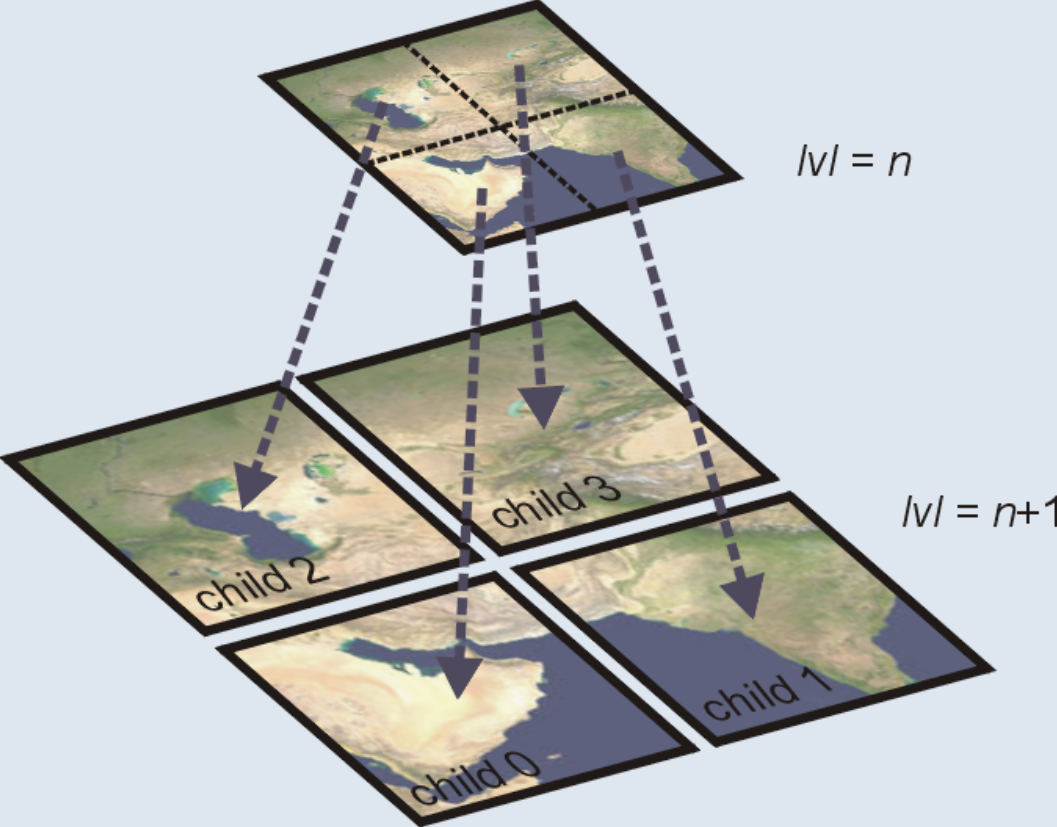
\includegraphics[width=0.5\textwidth]{quad_tree_tile.png}}
	\caption{Quadtree tile subdivision and child tiles at the next resolution level.}
\end{figure}

\noindent
The quadtree doesn’t need to be populated completely. Missing tiles are interpolated by Orbiter from a sub-area of an ancestor tile. The quadtree is also allowed to contain gaps, that is, it can contain high-resolution tiles of an area (e.g. a surface base) even if some of the ancestor tiles are missing from the tree, so that there is no unbroken chain to the quadtree root.\\
The minimum requirement is the presence of all tiles for resolution levels 1 to 4 for a given layer, i.e. the global tiles (level 1–3) and the quadtree root (level 4) must be present. All higher resolution quadtree tiles are optional. The maximum currently supported resolution level is 17 for elevation layers (Elev and Elev\_mod), and level 19 for all other layers.



\subsubsection{Layer types}
\subsubsection{Compressed archive layer format}
%\subsubsubsection{The .tree file format}
\subsubsection{Utilities}
\subsubsection{Elevation tile file format}
\subsubsection{Label tile format}
\subsubsection{Converting surface base tiles}



\subsection{Planet modules}
Planet modules can be used to control the motion of a planet (or any other celestial body, such as a moon, the sun, or an asteroid) within the solar system. This allows to implement sophisticated analytic ephemerides solutions which take into account perturbations from other celestial objects.\\
Planets which are not controlled via a DLL module are updated directly by Orbiter. Depending on the settings in the definition file, Orbiter either uses an unperturbed 2-body approximation, resulting in a conic section trajectory (e.g. an ellipse), or uses a dynamic update procedure based on the gravitational forces acting on the planet. Both methods have limitations: the 2-body approach ignores perturbations and is only valid if no massive bodies other than the orbit reference object are nearby. The dynamic update accumulates numerical errors over time, causing the orbits slowly to diverge from the correct trajectories.\\
By using a planet module, analytic perturbation solutions can be used which avoid the short-comings of the methods described above. Perturbation solutions typically describe the perturbed orbit of a planet by expressing the state vectors as a trigonometric series. These series are valid over a limited period of time, after which they start to diverge. Examples of perturbation solutions used in Orbiter are the VSOP87 solution for the 8 major planets and the sun, or the ELP2000 solution for the moon.\\
Planet modules can also define an atmosphere model for the celestial body. Atmosphere models return atmospheric data (temperature, density and pressure) at a specified altitude (and other optional parameters, such as geographic position and time). Atmospheric models can be implemented either directly in the planet module, or in a separate plugin module. Putting the atmosphere model into a separate plugin makes it easier to swap models later.\\
The following sections give a brief introduction into the design of planet modules. A general knowledge of writing orbiter plugins is assumed.

\subsubsection{First steps}
Create a new DLL project for your planet module, e.g. in \textit{Orbitersdk\textbackslash samples\textbackslash MyPlanet}. Set up all the usual include and library paths for Orbiter plugins. Add \textit{orbiter.lib} and \textit{orbitersdk.lib} as additional dependencies.

\subsubsection{The CELBODY2 interface class}
The communication between the Orbiter core and the planet module is performed via callback functions defined in the \textit{CELBODY} and \textit{CELBODY2} classes. (\textit{CELBODY2} is derived from \textit{CELBODY} and contains all the properties of the base class, plus a significantly extended atmospheric parameter interface). The \textit{CELBODY} interface is retained for backward compatibility, but all new planet modules should refer to the \textit{CELBODY2} interface.\\
We now need to the class interface for the new planet module by deriving a custom class from \textit{CELBODY2}. Create a new header file in your project, e.g. \textit{MyPlanet.h}, and add the following:

\begin{lstlisting}
#include "OrbiterAPI.h"
#include "CelbodyAPI.h"

class DLLEXPORT MyPlanet:public CELBODY2
{
	public:
		MyPlanet( OBJHANDLE hObj );
		void clbkInit( FILEHANDLE cfg );
		int clbkEphemeris( double mjd, int req, double* ret );
		int clbkFastEphemeris( double simt, int req, double* ret );
};
\end{lstlisting}

\noindent
\textit{OrbiterAPI.h} contains the general API interface, and \textit{CelbodyAPI.h} contains the planet module-specific interface, in particular the \textit{CELBODY}, \textit{CELBODY2} and \textit{ATMOSPHERE} classes.\\
The \textit{clbkEphemeris} and \textit{clbkFastEphemeris} methods are callback functions which Orbiter will call whenever the planet positions and velocities ("ephemerides") need to be updated. They will be described in more detail below. The clbkInit method is called by Orbiter after the planet module has been loaded. It receives a file handle for the planet's configuration file. This allows the module to read configuration parameters from the file.\\
%TODO reference API manual?
The \textit{CELBODY2} interface contains a few more methods related to defining an atmospheric model. These will be discussed below. Check the API Reference manual for a complete list of class methods.\\
To implement the methods in our \textit{MyPlanet} class, create a source file in your project, e.g. \textit{MyPlanet.cpp}. Add the following lines:

\begin{lstlisting}
#define ORBITER_MODULE
#include "MyPlanet.h"

MyPlanet::MyPlanet( OBJHANDLE hObj ):CELBODY2( hObj )
{
	// add constructor code here
}

void MyPlanet::clbkInit( FILEHANDLE cfg )
{
	/*
	read parameters from config file (e.g. tolerance limits, etc)
	perform any required initialisation (e.g. read perturbation
		terms from data files)
	*/
}

bool MyPlanet::bEphemeris() const
{
	return true;
	// class supports ephemeris calculation
}

int clbkEphemeris( double mjd, int req, double* ret )
{
	// return planet position and velocity for Modified Julian date mjd in ret
}

int clbkFastEphemeris( double simt, int req, double* ret )
{
	/*
	return interpolated planet position and velocity
		for simulation time simt in ret
	*/
}
\end{lstlisting}

\noindent
The first line defining \textit{ORBITER\_MODULE} is required to ensure that all initialisation functions are properly called by Orbiter.\\
\textit{clbkEphemeris} and \textit{clbkFastEphemeris} are the functions which will contain the actual ephemeris calculations for the planet at the requested time. \textit{clbkEphemeris} is only called by Orbiter if the planet’s state at an arbitrary time is required (for example by an instrument calculating the position at some future time). When Orbiter updates the planet’s position for the next simulation time frame, the \textit{clbkFastEphemeris} function will be called instead. This means that \textit{clbkFastEphemeris} will be called at each frame, each time advancing the time by a small amount. This can be used for a more efficient calculation. Instead of performing a full series evaluation, which can be lengthy, you may implement an interpolation scheme which performs the full calculation only occasionally, and interpolates between these samples to return the state at an intermediate time.\\
For both functions, the requested type of data is specified as a group of \textit{EPHEM\_xxx} bitflags in the \textit{req} parameter. This can be any combination of position and velocity data for the celestial body itself and/or the barycentre of the system defined by the body and all its children (moons). The functions should calculate all required data, either in cartesian or polar coordinates, and fill the \textit{ret} array with the results. \textit{ret} contains 12 entries, used as follows:

\begin{itemize}
\item ret[0-2] $\Rightarrow$ true position
\item ret[3-5] $\Rightarrow$ true velocity
\item ret[6-8] $\Rightarrow$ barycentric position
\item ret[9-11] $\Rightarrow$ barycentric velocity
\end{itemize}

\noindent
Only the fields requested by \textit{req} need to be filled. In cartesian coordinates, the position fields must contain the x, y and z coordinates in [m], and the velocity fields must contain the velocities d\textit{x}/d\textit{t}, d\textit{y}/d\textit{t}, d\textit{z}/d\textit{t} in [m/s]. In spherical polar coordinates, the position fields must contain longitude $\phi$ [rad], latitude $\theta$ [rad] and radial distance \textit{r} [AU], and the velocity fields must contain the polar velocities d$\phi$/dt [rad/s], d$\theta$/dt [rad/s] and d\textit{r}/d\textit{t} [AU/s].\\
The functions should indicate the fields actually calculated via the return value. This is in particular important if not all requests could be satisfied (e.g. position and velocity was requested, but only position could be calculated). The return value is interpreted as a bitflag that can contain the same \textit{EPHEM\_xxx} flags as the \textit{req} parameter. If all requests could be satisfied, it should be identical to \textit{req}. In addition, the return value should contain additional flags indicating the properties of the returned data, including \textit{EPHEM\_POLAR} if the data are returned as spherical polar coordinates, or \textit{EPHEM\_TRUEISBARY} if the true and barycentric coordinates are identical (i.e. the celestial body does not have child bodies).


\subsubsection{The API interface}
Next, we need to define the API interface that will allow Orbiter to load an instance of the celestial body interface. This is done by implementing the \textit{InitInstance} and \textit{ExitInstance} functions in \textit{MyPlanet.cpp}:

%TODO shouldn't this be CELBODY2?
\begin{lstlisting}
DLLCKBK CELBODY* InitInstance( OBJHANDLE hBody )
{
	// instance initialisation
	return new MyPlanet;
}

DLLCLBK void ExitInstance( CELBODY* body )
{
	// instance cleanup
	delete (MyPlanet*)body;
}
\end{lstlisting}

\noindent
\textit{InitInstance} and \textit{ExitInstance} are called by Orbiter each time an instance of the planet is loaded or discarded. There are also functions \textit{InitModule} and \textit{ExitModule}, which are called only once per simulation run, and can be used to initialise and clean up global resources:

\begin{lstlisting}
DLLCLBK void InitModule( HINSTANCE hModule )
{
	// module initialisation
}

DLLCLBK void ExitModule( HINSTANCE hModule )
{
	// module cleanup
}
\end{lstlisting}

\noindent
Because usually only a single instance of a specific planet object is created during a simulation, the difference between \textit{InitInstance} and \textit{InitModule} is not as significant here as it is for vessel modules. The \textit{InitModule} and \textit{ExitModule} methods can be omitted if the module doesn’t need any global parameter initialisation.


\subsection{Defining an atmosphere}
Planetary atmospheres have a significant influence on the flight behavior of spacecraft. The primary atmospheric parameters are temperature, pressure and density as a function of altitude.\\
Defining a simple atmospheric model is possible by setting a few parameters in the planet’s configuration file. More sophisticated models must be coded in the planet’s DLL module.\\
Orbiter currently does not model local atmospheric perturbations (climatic/weather effects), although local temperature and pressure variations can be implemented by customised atmosphere models.


\subsubsection{A simple atmosphere}
To define a simple exponentially decaying atmosphere, define the following items in the planet’s configuration (.cfg) file:

\begin{itemize}
\item AtmPressure0 $\Rightarrow$ The static atmospheric pressure [Pa] at altitude zero, $p_{0}$.
\item AtmDensity0 $\Rightarrow$ The atmospheric density [kg/m$^{3}$] at altitude zero, $\rho_{0}$.
\item AtmAltLimit $\Rightarrow$ The altitude above which atmospheric effects can be neglected.
\end{itemize}

\noindent
where altitude zero is defined as distance \textit{Size} (as defined in the configuration file) from the planet’s centre.\\
The pressure and density at any altitude h is then calculated by Orbiter as

\[ p =
\left\{
\begin{array}{ll}
	p_{0}e^{-Ch} & h \leq AtmLimit \\
	0 & otherwise \\
\end{array} 
\right. \]

\[ \rho =
\left\{
\begin{array}{ll}
	\rho_{0}e^{-Ch} & h \leq AtmLimit \\
	0 & otherwise \\
\end{array} 
\right. \]

\noindent
where $C = \frac{\rho_{0}}{p_{0}}g_{0}$, and $g_{0}$ is the gravitational acceleration at altitude zero.\\
This model assumes constant temperature.


\subsubsection{A more sophisticated atmosphere}
%TODO add section link
Where the simple model described above is not adequate, a more detailed atmospheric model can be implemented in a plugin module. This section assumes that a module for the celestial body has already been created, as outlined in Section TODO.\\
The atmosphere model interface is described by the \textit{ATMOSPHERE} class defined in \textit{CelbodyAPI.h}. To create a custom atmosphere model, create a new header file in your planet project, e.g. \textit{MyAtmosphere.h}. The atmosphere class interface should look like

\begin{lstlisting}
#include "OrbiterAPI.h"
#include "CelbodyAPI.h"

class DLLEXPORT MyAtmosphere: public ATMOSPHERE
{
	public:
		MyAtmosphere( CELBODY2* body );
		const char* clbkName() const;
		bool clbkConstants( ATMCONST* atmc ) const;
		bool clbkParams( const PRM_IN* prm_in, PRM_OUT* prm_out );
};
\end{lstlisting}

\noindent
The constructor takes the \textit{CELBODY2} class instance of the associated celestial body as a parameter.\\
The \textit{clbkName} callback function should return a short name identifying the model.\\
\\
The \textit{clbkConstants} callback function should return in \textit{atmc} some basic atmosphere parameters, such as the mean density and pressure at ground level, gas constant and ratio of specific heats, as well as some rendering parameters.\\
Note that some of the parameters returned by \textit{clbkConstants} may be overwritten by the settings defined in the celestial body's configuration file. Configuration file entries take precedence over \textit{clbkConstants}.\\
The \textit{clbkParams} callback function should return atmospheric temperature, density and pressure at the location specified by the data in the \textit{prm\_in} parameter. Simple models may depend on altitude only, but more sophisticated models can make use of the additional parameters such as position (longitude and latitude), solar flux, geomagnetic index, and date.\\
Create a source file, e.g. \textit{MyAtmosphere.cpp}, to implement the actual model. A very simplistic implementation may look like this:

\begin{lstlisting}
#include "MyAtmosphere.h"

static double T0       = 288.0;  // ground level temperature [K]
static double p0       = 101325; // ground level pressure [Pa]
static double rho0     = 1.2250; // ground level density [kg/m^3]
static double R        = 286.91; // gas constant
static double gamma    = 1.4;    // ratio of specific heats
static double altlimit = 200e3;  // cutoff altitude
static double C        = rho0 / p0;

MyAtmosphere::MyAtmosphere( CELBODY2* body ):ATMOSPHERE( body )
{
}

const char* MyAtmosphere::clbkName() const
{
	static char* name = "Simple";
	return name;
}

bool MyAtmosphere::clbkConstants( ATMCONST* atmc ) const
{
	atmc->p0 = p0;
	atmc->rho0 = rho0;
	atmc->R = R;
	atmc->gamma = gamma;
	atmc->altlimit = altlimit;
	return true;
}

bool MyAtmosphere::clbkParams( const PRM_IN* prm_in, PRM_OUT* prm_out )
{
	double z = (prm_in->flag & PRM_ALT ? prm_in->alt : 0.0);
	if (z < 200e3)
	{
		double scale = exp( -C * z );
		prm_out->T = T0;
		prm_out->rho = rho0 * scale;
		prm_out->p = p0 * scale;
		return true;
	}
	else
	{
		prm_out->T = 0;
		prm_out->rho = 0;
		prm_out->p = 0;
		return false;
	}
}
\end{lstlisting}

\noindent
%TODO add tech note earth atm link
The above example serves only as an illustration. The actual atmosphere models provided with the Orbiter distribution are more complex. For some background on the supported Earth atmosphere models, see the technical note in TODO.\\
Now we need to link the atmosphere model into the celestial body interface. This can be done with the \textit{SetAtmosphere} function of the \textit{CELBODY2} class. Add the following statement to the \textit{clbkInit} method of your \textit{MyPlanet} definition:

\begin{lstlisting}
#include "MyAtmosphere.h"

void MyPlanet::clbkInit( FILEHANDLE cfg )
{
	SetAtmosphere( new MyAtmosphere( this ) );
}
\end{lstlisting}

\noindent
The atmosphere instance will be destroyed automatically when the planet instance is deleted.


\subsubsection{External atmosphere modules}
Instead of implementing the atmosphere model inside the planet module, it can can also be implemented in a separate plugin module. This makes it easier to exchange the atmosphere model for a different one later on, without having to have access to the rest of the planet module code.\\
To implement the atmosphere as a separate module, create a new DLL project for it. Add the \textit{MyAtmosphere.h} and \textit{MyAtmosphere.cpp} files created in the previous section to the project. Since the atmosphere is now defined in its own module, add the line

\begin{lstlisting}
#define ORBITER_MODULE

\end{lstlisting}

\noindent
on top of \textit{MyAtmosphere.cpp}.\\
In addition, you need to define an API interface to the module code. It should look like this:

\begin{lstlisting}
DLLCLBK void InitModule( HINSTANCE hModule )
{
	// module initialisation
}

DLLCLBK void ExitModule( HINSTANCE hModule )
{
	// module cleanup
}

DLLCLBK ATMOSPHERE* CreateAtmosphere( CELBODY2* cbody )
{
	return new MyAtmosphere( cbody );
}

DLLCLBK void DeleteAtmosphere( ATMOSPHERE* atm )
{
	delete (MyAtmosphere*)atm;
}
\end{lstlisting}

\noindent
By convention, external planetary atmosphere modules should be placed in the\\
\indent \textit{Modules\textbackslash Celbody\textbackslash <Name>\textbackslash Atmosphere}\\
folder, where <\textit{Name}> is the celestial body's name. So in our case,\\
\indent \textit{Modules\textbackslash Celbody\textbackslash MyPlanet\textbackslash Atmosphere\textbackslash MyAtmosphere.dll}\\
We now need to modify the \textit{MyPlanet} code to allow it to load its atmosphere interface from an external module. Replace the \textit{SetAtmosphere} statement in the \textit{clbkInit} function with

\begin{lstlisting}
void MyPlanet::clbkInit( FILEHANDLE cfg )
{
	LoadAtmosphereModule( "MyAtmosphere" );
}
\end{lstlisting}

\noindent
However, this causes the atmospheric module name to be hardcoded in the planet module. A more flexible method is to specify the atmospheric module in the celestial body's configuration file, using the \textit{MODULE\_ATM} entry. Our \textit{MyPlanet.cfg} file might look like this:

\begin{lstlisting}[language=OSFS]
NAME = MyPlanet
MODULE = MyPlanet
MODULE_ATM = MyAtmosphere
\end{lstlisting}

\noindent
If the \textit{MODULE\_ATM} entry is defined in the configuration file, then the default \textit{CELBODY2::clbkInit} implementation will load the atmosphere module directly, so we only need to make sure to call the base class method:

\begin{lstlisting}
void MyPlanet::clbkInit( FILEHANDLE cfg )
{
	CELBODY2::clbkInit( cfg );
}
\end{lstlisting}

\noindent
Calling the \textit{CELBODY2::clbkInit} method also enables another interesting feature: Before reading the \textit{MODULE\_ATM} entry in the planet configuration file, Orbiter scans the \textit{Config\textbackslash <Name>\textbackslash Atmosphere.cfg} file for an entry "Model" and uses that, if present. This file is written by the \textit{Atmosphere configuration tool} in the Extra tab of the Orbiter launchpad, which provides a convenient method for users to change atmosphere models. This mechanism allows to add new atmosphere modules without the need to change any configuration files. As long as the atmosphere DLL modules are placed in the correct location (\textit{Modules\textbackslash Celbody\textbackslash <Name>\textbackslash Atmosphere}), they will be scanned automatically by the atmosphere selector tool.


\subsubsection{Adding and replacing atmosphere models}
Most of the celestial body modules in the default Orbiter distribution have built-in support for external atmosphere modules, and some of them (Earth, Mars and Venus) come with one or several atmosphere modules. To add additional choices for atmosphere models for a body, create one as outlined above, and simply drop the DLL library into the \textit{Modules\textbackslash Celbody\textbackslash <Name>\textbackslash Atmosphere} folder. If that folder doesn't exist yet, you have to create it. The user can then select the new model from the Extra tab in the Orbiter Launchpad (Celestial body configuration | Atmosphere configuration).\\
For best support of the atmosphere model selection tool, your atmosphere module should contain two additional API functions:

\begin{lstlisting}
DLLCLBK char* ModelName()
{
	static char* name = "MyAtmosphere";
	return name;
}

DLLCLBK char* ModelDesc()
{
	static char* desc = "My custom atmosphere model";
	return desc;
}
\end{lstlisting}

\noindent
The string returned by the \textit{ModelName} function represents the model in the dialog's selection list box. The string returned by \textit{ModelDesc} should contain a short description (max 256 characters displayed in the dialog box when the model is selected.\\
If you don't want to design your own custom atmosphere model, you can quickly add atmospheres to planets by replicating existing ones. Simply copy an atmosphere module from the\\
\indent \textit{Modules\textbackslash Celbody\textbackslash <Name>\textbackslash Atmosphere}\\
folder of one planet to that of another one. It then becomes available in the list of atmospheres for that planet. Note that the module only provides the physical atmospheric parameters. You will still have to edit the definition file to provide visual effects.\\
Of course, replicating an atmosphere should be regarded as a quick and dirty trick for experimentation. Atmospheres are always tailor-made for specific bodies, and don't realistically fit anywhere else.


\subsubsection{Earth default atmosphere models}
%TODO add tech note earth atm link
The Orbiter distribution contains three Earth atmosphere models that can be selected by the user from the Extra tab in the Launchpad dialog. See TODO for further details on the different models.\\
\textbf{Jacchia71-Gill Atmosphere Model.} This is an implementation of the Jacchia-71 (J71) model\cite{jacchia71}, using a polynomial series approximation by Gill\cite{gill96}. It uses a static US Standard Atmosphere model below 90km, and a diffusion-equilibrium solution be­tween 90 and 2500km altitude. The only model parameter is the exospheric temperature.\\
\textbf{NRLMSISE-00 Atmosphere Model.} This model is based on the MSISE90 model, with the addition of further corrections based on observation data. MSISE90 provides the neutral temperature and density from ground level to thermospheric altitudes. Unlike the Jacchia models, the low-altitude data are not static, but vary with location.\\
\textbf{Orbiter 2006 Legacy model.} This is the model that was used in the Orbiter 2006 Edition. It is based on a static standard model\cite{anderson2000} below 105km, and assumes constant temperature and exponentially decaying density and pressure between 105 and 200km. This model underestimates density and pressure above $\sim$120km, which reduces the orbit decay of object in low Earth orbit.\\
In addition, the atmosphere can be disabled for testing/debugging purposes.

\subsubsection{Mars atmosphere}
Orbiter uses the following atmospheric parameter profiles for Mars:

%\begin{table}[H]
	%\centering
	\begin{longtable}{ |p{0.2\textwidth}|p{0.1\textwidth}|p{0.1\textwidth}|p{0.1\textwidth}|p{0.1\textwidth}|p{0.1\textwidth}|p{0.1\textwidth}| }
	\hline\rule{0pt}{2ex}
	Altitude [km] & 0 & 2 & 4 & 14 & 20 & 30\\
	\hline\rule{0pt}{2ex}
	Temperature [K] & 195 & 200 & 200 & 180 & 180 & 165\\
	\hline\rule{0pt}{2ex}
	Pressure [Pa] & 610.0 & 499.5 & 410.1 & 145.1 & 75.2 & 23.9\\
	\hline\rule{0pt}{2ex}
	Density [kg m$^{-3}$] & 0.02 & 0.0160 & 0.0131 & 0.0052 & 2.7$\cdot$10$^{-3}$ & 9.3$\cdot$10$^{-4}$\\
	\hline
	\end{longtable}
%\end{table}

\noindent
\begin{figure}[H]
	\centering
	\subfigure{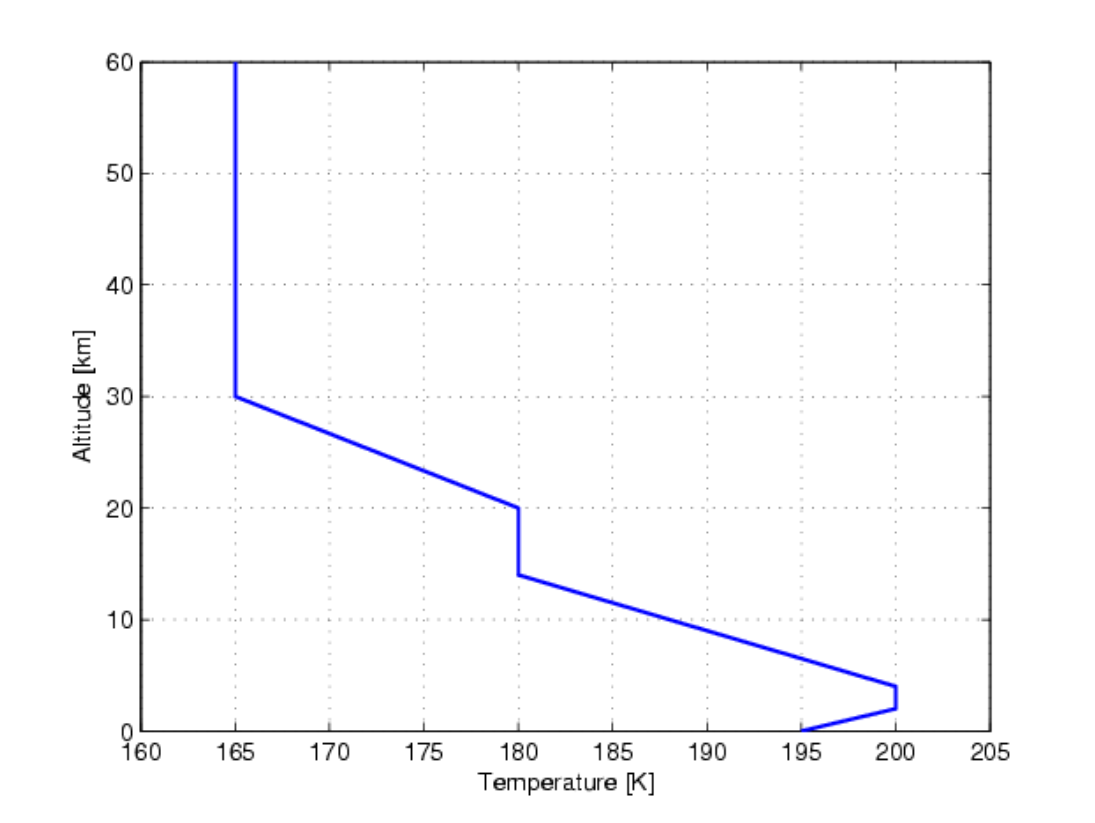
\includegraphics[width=0.49\textwidth]{mars_atm_temperature.png}}
	\subfigure{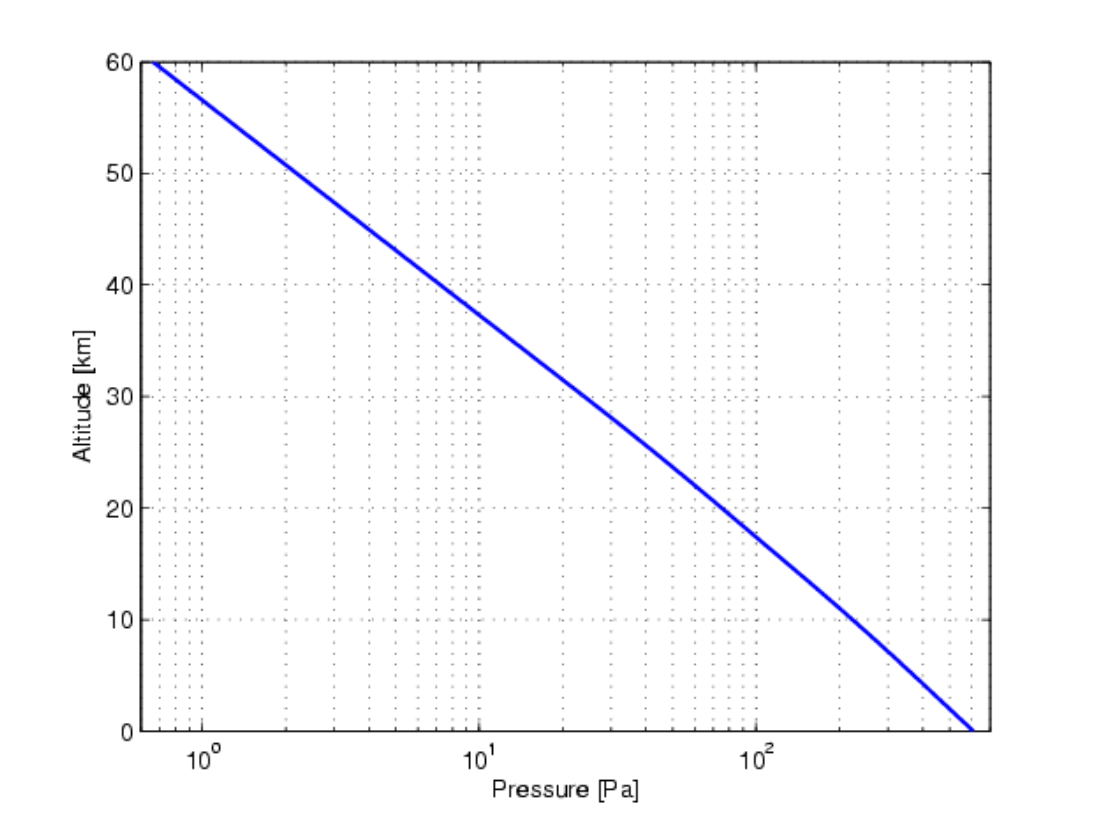
\includegraphics[width=0.49\textwidth]{mars_atm_pressure.png}}
	\subfigure{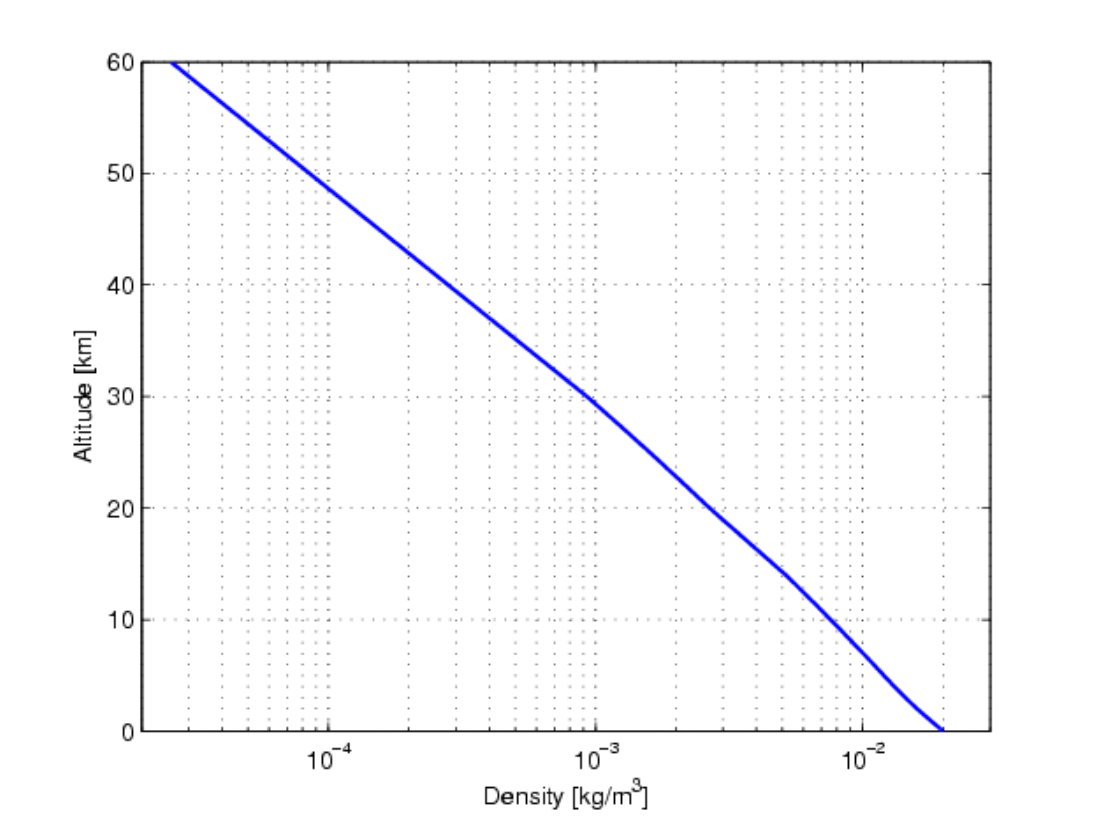
\includegraphics[width=0.49\textwidth]{mars_atm_density.png}}
\end{figure}

\noindent
Atmospheric parameters:

\begin{itemize}
\item Surface pressure: $p_{0}$ = 610.0 Pa
\item Surface density: $\rho_{0}$ = 0.020 kg m$^{-3}$
\item Ratio of specific heats: $\gamma$ = 1.2941
\item Specific gas constant: \textit{R} = 188.92 J K$^{-1}$ kg$^{-1}$
\end{itemize}

\noindent
Orbiter defines the upper atmosphere altitude limit as 100 km.


\subsubsection{Venus atmosphere}
Orbiter uses the following atmospheric parameter profiles for Venus:

%\begin{table}[H]
	%\centering
	\begin{longtable}{ |p{0.2\textwidth}|p{0.1\textwidth}|p{0.1\textwidth}|p{0.1\textwidth}|p{0.1\textwidth}|p{0.1\textwidth}|p{0.1\textwidth}| }
	\hline\rule{0pt}{2ex}
	Altitude [km] & 0 & 30 & 60 & 70 & 90 & 200\\
	\hline\rule{0pt}{2ex}
	Temperature [K] & 750 & 480 & 230 & 230 & 180 & 180\\
	\hline\rule{0pt}{2ex}
	Pressure [Pa] & 9.2M & 897k & 14.2k & 1.85k & 18.5 & 3.4$\cdot$10$^{-11}$\\
	\hline\rule{0pt}{2ex}
	Density [kg m$^{-3}$] & 65 & 9.9 & 0.33 & 0.043 & 5.4$\cdot$10$^{-4}$ & 1.0$\cdot$10$^{-15}$\\
	\hline
	\end{longtable}
%\end{table}

\noindent
\begin{figure}[H]
	\centering
	\subfigure{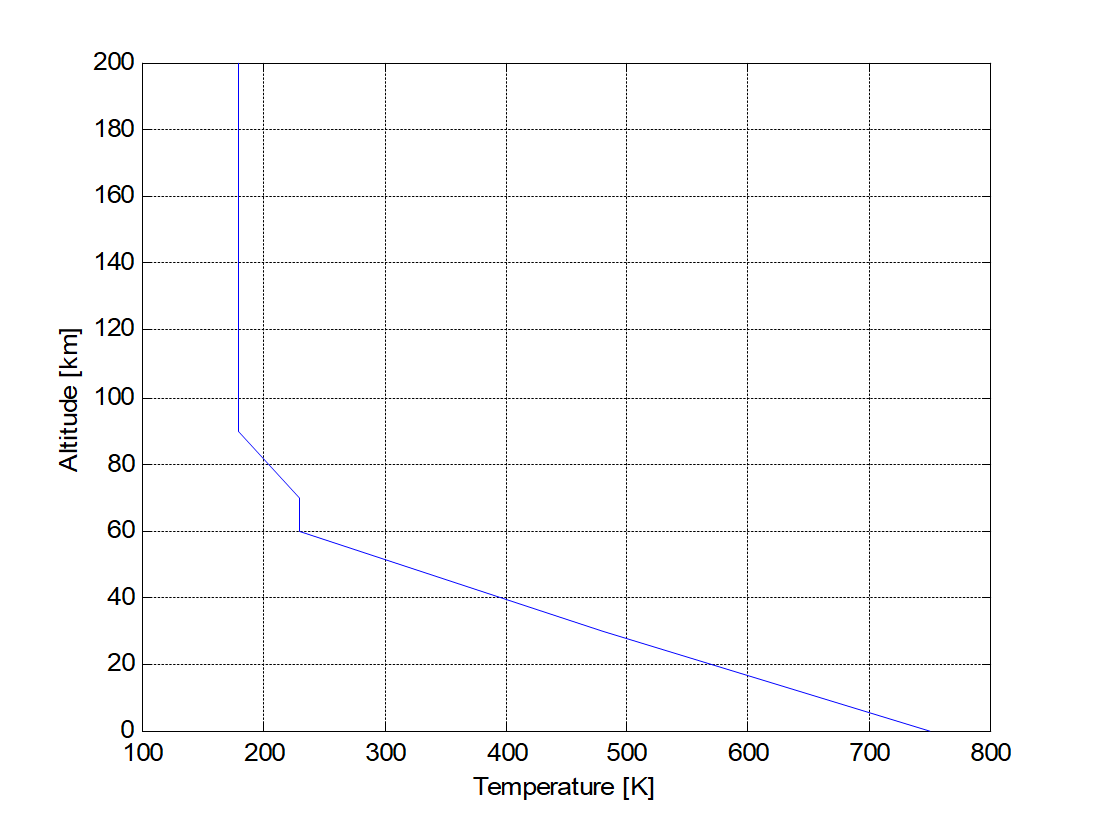
\includegraphics[width=0.49\textwidth]{venus_atm_temperature.png}}
	\subfigure{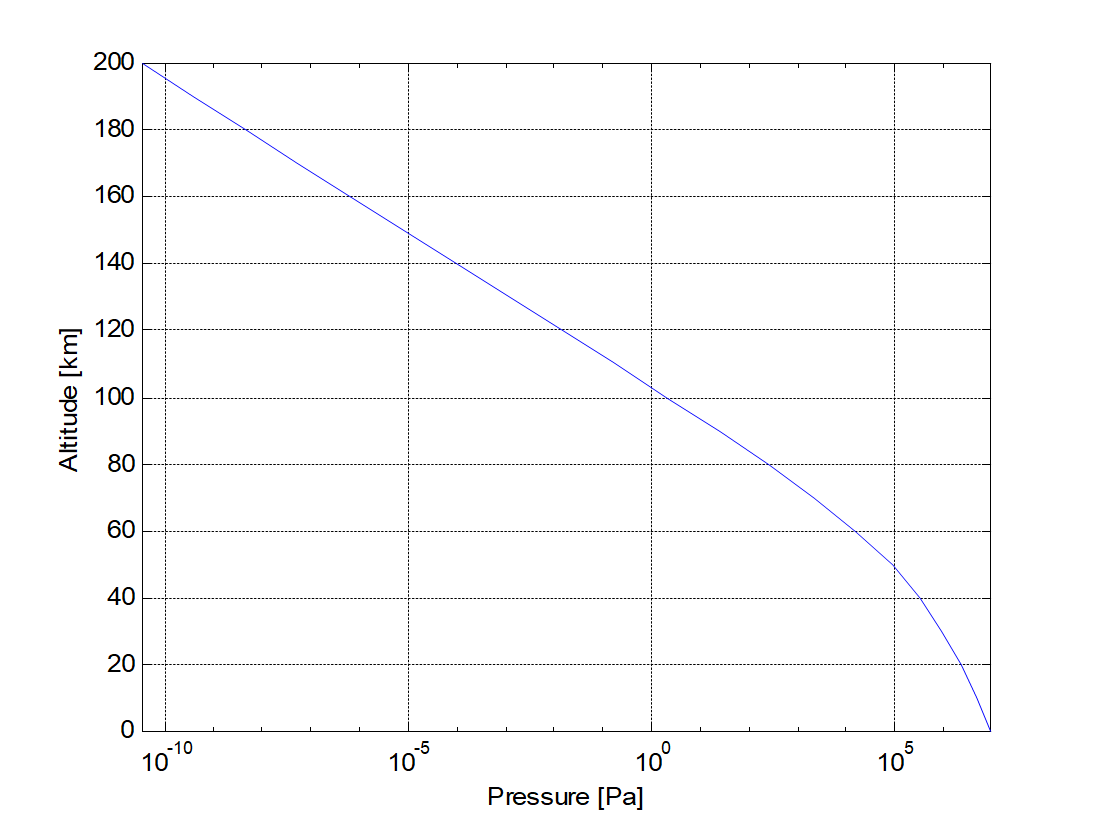
\includegraphics[width=0.49\textwidth]{venus_atm_pressure.png}}
	\subfigure{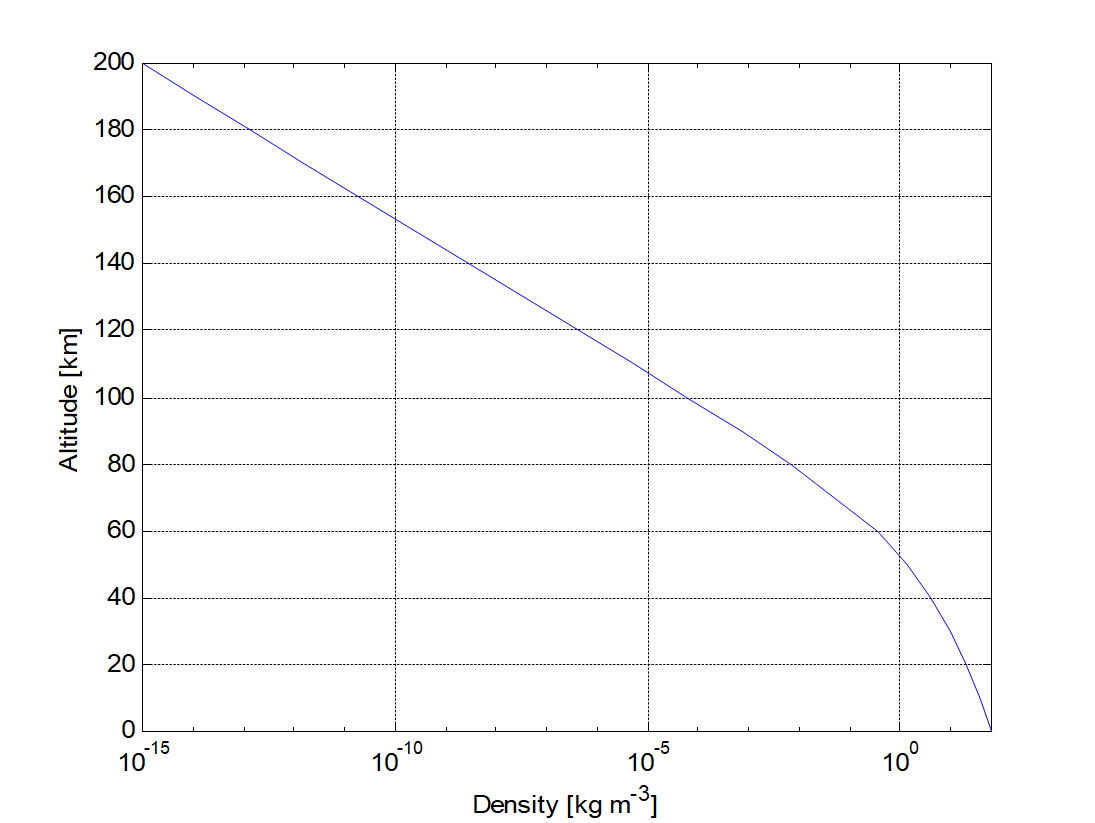
\includegraphics[width=0.49\textwidth]{venus_atm_density.png}}
\end{figure}

\noindent
Atmospheric parameters:

\begin{itemize}
\item Surface pressure: $p_{0}$ = 9.2 MPa
\item Surface density: $\rho_{0}$ = 65 kg m$^{-3}$
\item Ratio of specific heats: $\gamma$ = 1.2857
\item Specific gas constant: \textit{R} = 188.92 J K$^{-1}$ kg$^{-1}$
\end{itemize}

\noindent
Orbiter defines the upper atmosphere altitude limit as 200 km. The cloud layer is set at an altitude of 60 km.


\subsubsection{The speed of sound}
Orbiter uses the equation for an ideal gas to compute the speed of sound as a function of absolute temperature:

\[ a = \sqrt{\gamma RT} \]

\noindent
where $\gamma$ is the ratio of specific heat at constant pressure $c_{p}$, and specific heat at constant temperature, $c_{v}$, for the gas, $\gamma = c_{p} / c_{v}$ For air at normal conditions, $\gamma$ = 1.4. This value is used by Orbiter as a default. It can be overridden by setting the \textit{AtmGamma} parameter in the planet’s configuration file.\\
\textit{R} is the specific gas constant. By default, Orbiter uses the value for air, 286.91 J K$^{-1}$ kg$^{-1}$. This can be overridden by setting the \textit{AtmGasConstant} parameter in the planet’s configuration file.\\
\textbf{Mach number:} The Mach number is an essential parameter in aerodynamics. It expresses a velocity \textit{v} in units of the current speed of sound:

\[ M = \frac{v}{a} \]


\end{document}
